In this section you will find an evaluation of the different algorithms, including experiments with various parameters for them and comparison to existing solutions from Section \ref{sec:stateoftheart}.

\section{Methodology}
Audio compression quality is most often evaluated using a series of listening tests (such as the one pictured in Figure \ref{fig:opus_listening_test}). However, due to a lack of resources to conduct such a thing, a different method must be used - although they are generally not as accurate.

One of the most used methods for objectively evaluating perceptible audio quality is PEAQ \cite{peaq_2006}, however its specifications are insufficient, and its implementations proprietary. The exact algorithm and parameters aren't known for the most part. It comes in two variants:

\begin{description}
	\item[PEAQ Basic] intended for real-time use
	\item[PEAQ Advanced] a more comprehensive model, intended for non real-time use
\end{description}

Even though neither of these is directly available, luckily, there are a few open-source alternatives that try to implement similar algorithms, with their quality measured by comparing their output to PEAQ, and by proxy, to listening tests.

One of the more prominent open-source solutions is GstPEAQ, which according to its paper \cite{gstpeaq_paper} performs better than the other implementations. So while it does not conform to the PEAQ recommendation directly, its results are within an acceptable margin and thus this thesis will use GstPEAQ for quality evaluation.

\section{GstPEAQ}
GstPEAQ is a plugin for GStreamer \cite{gstreamer_2016} (a pipeline-based multimedia framework) and its source code is freely available at \cite{gstpeaq_impl}. It implements both the Basic and Advanced mode of PEAQ as specified in \cite{peaq_2006}, however as the standard is under-specified, educated guesses must be taken at points.

It's also important to mention that I could not get the Advanced mode to work without errors, and as such testing will be performed in Basic mode only.

And just like PEAQ, the algorithm's main output is a value known as \emph{Objective Difference Grade} (ODG), which evaluates the perceptible impairment (quality difference) between the provided audio and the reference audio. It uses various psychoacoustic "features" of the signal to determine the grade, the details of which won't be covered here - please refer to either paper for specifics.

The ODG scale contains real values from $0$ to $-4$, ranging from imperceptible difference to very annoying for the human ear. Please refer to Table \ref{tab:odg_scale} to see the full scale.

\begin{table}[htbp]\caption{PEAQ - Objective Difference Grade table}
	\label{tab:odg_scale}
	\centering
	\begin{tabular}{|c|l|}
		\hline
		ODG & Impairment description \\ \hline
		$0.0$ & Imperceptible \\
		$-1.0$ & Perceptible, but not annoying \\
		$-2.0$ & Slightly annoying \\
		$-3.0$ & Annoying \\
		$-4.0$ & Very annoying \\
		\hline
	\end{tabular}
\end{table}

\section{Evaluating results}
In this section we will experiment with various parameters for all the encoding methods, find a good compromise between bitrate and ODG, and then compare those results to the reference codings (MP3, Opus) at similar bitrates.

The evaluating process will work in these steps:

\begin{enumerate}
	\item compress example WAV file using ANMF
	\item decompress ANMF back to a WAV file
	\item measure ODG between old and new WAV file
\end{enumerate}

In the case of MP3 or Opus files, they will be decoded to WAV for comparison.

\subsection{Audio examples}
There's a total of four example audio files in WAV format that will be used for testing. Please refer to Table \ref{tab:audio_examples} for a list. All of the examples are $\sim5-10$ second excerpts from audio files using 44.1 kHz sampling rate and 16-bit signed integer samples. These files can be found in the \verb|examples| folder of the implementation.

\begin{table}[htbp]\caption{List of tested audio files}
	\label{tab:audio_examples}
	\centering
	\begin{tabular}{|c|c|c|c|l|}
		\hline
		ID & File name & Description \\ \hline
		$00$ & \verb|piano16t.wav| & Clear sounding piano sounds \\
		$01$ & \verb|henry16t.wav| & Average quality English voice \\
		$02$ & \verb|swave16t.wav| & Simple electronic music \\
		$03$ & \verb|taleena16t.wav| & Complex music including lyrics \\
		\hline
	\end{tabular}
\end{table}

\subsection{Bitrate}
The bitrate is the amount of bits that a computer needs to process per a unit of time, in this context it means how many bits are needed to play back 1 second of an audio file.

To find the bitrate of a WAV file with a sampling rate $F_s$, we can use the following equation:

\begin{align}
bitrate = channelCount \cdot F_s \cdot bitsPerSample
\end{align}

So in regards to compressing the example files, our target bitrate is at most $2 \cdot 44100 \cdot 16 = 1411200$ bits per second (or $\sim 1411$ kbps).

To calculate the number of elements in an NMF-approximated matrix $V$ of size $m \times n$ with approximation rank $r$, we can use the following equation:

\begin{align}
\label{equ:nmf_size}
size(NMF(V)) = r(m+n)
\end{align}

\emph{Proof:} NMF approximates a matrix $m \times n$ into two matrices $m \times r$ and $r \times n$, therefore the total size is $mr + rn = r(m+n)$.

\subsection{ANMF-RAW}
For ANMF-RAW, we need to find a compromise between the size of one chunk and the rank of the NMF. First, we'll fix the shape to $1152 \times 200$ and experiment with the rank.

The maximum number of iterations has been fixed to 3000, since past that point the cost function is almost stable as seen in Figure \ref{fig:anmf_raw_cost_func}.

\begin{figure}[ht]
	\caption[ANMF-RAW cost function]{The value of the cost function per iteration during NMF in ANMF-RAW at rank $= 30$.}
	\label{fig:anmf_raw_cost_func}
	\centering
	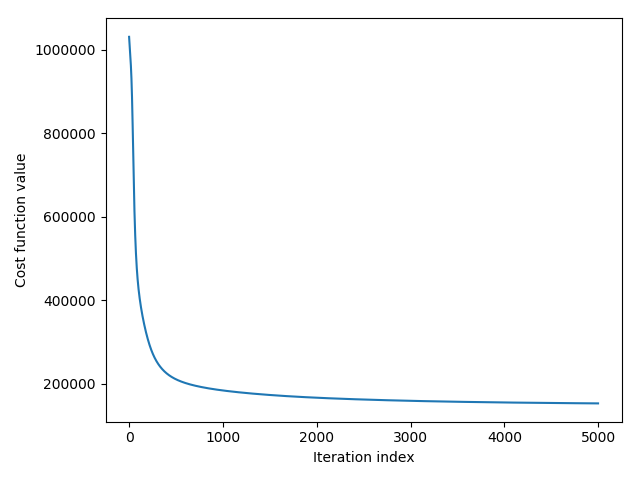
\includegraphics[width=\textwidth]{anmf_raw_cost_func.png}
\end{figure}

In Table \ref{tab:anmf_raw_rank}, you can see the results of changing the rank of the NMF approximation. The rows correspond to the example IDs from Table \ref{tab:audio_examples}, and the columns correspond to the ODG for different rank values.

\begin{table}[htbp]\caption{ANMF-RAW rank experiment results}
	\label{tab:anmf_raw_rank}
	\centering
	\begin{tabular}{|c|c|c|c|c|c|}
		\hline
		ID & rank 30 & rank 40 & rank 45 & rank 60 & rank 75 \\ \hline
		$00$ & $-3.873$ & $-3.830$ & $-3.811$ & $-3.749$ & $-3.650$ \\
		$01$ & $-3.908$ & $-3.902$ & $-3.895$ & $-3.861$ & $-3.844$ \\
		$02$ & $-3.868$ & $-3.850$ & $-3.837$ & $-3.800$ & $-3.759$ \\
		$03$ & $-3.744$ & $-3.519$ & $-3.361$ & $-2.825$ & $-2.461$ \\		
		\hline
	\end{tabular}
\end{table}

It's also worth mentioning that the runtime necessary for compression scales with the rank, as seen in Table \ref{tab:anmf_raw_runtime}.

\begin{table}[htbp]\caption{ANMF-RAW average runtime in seconds}
	\label{tab:anmf_raw_runtime}
	\centering
	\begin{tabular}{|c|c|c|c|c|c|}
		\hline
		ID & rank 30 & rank 40 & rank 45 & rank 60 & rank 75 \\ \hline
		$00$ & $63.378$s & $65.913$s & $67.082$s & $71.684$s & $75.839$s \\	
		\hline
	\end{tabular}
\end{table}

Interestingly enough, sample ID 03 notices the largest improvement despite being the more complex of the four, but when listening to the decompressed audio, it still sounds quite distorted and noticeable. Another looming issue is that at that rank the size of the compressed file approaches the original filesize, so we will need to lower the rank and try a lower chunk size instead.

To calculate the bitrate of ANMF-RAW, we must take into account the chunk size and the rank of the NMF approximation and then use Equation \ref{equ:nmf_size}. There is some overhead for the metadata, but as it spans only a few bytes it will be disregarded. The bitrate of ANMF-RAW with a chunk size of $m \times n$ and rank $r$ can be calculated as:

\begin{align}
bitrate^{RAW} = r(m+n) \cdot \frac{F_s}{mn} \cdot bitsPerValue \cdot channelCount
\end{align}

Therefore, for a chunk $1152 \times 200$ with rank 75, we get:

\begin{align}
bitrate^{RAW} = 75 \cdot (1152 + 200) \cdot \frac{44100}{1152 \cdot 200} \cdot 32 \cdot 2 = 1242150
\end{align}

Our target is 1411 kbps and our compression with 1242 kbps is judged as "annoying" by GstPEAQ. We will try lowering the chunk size and rank both to see if it has an effect. It was mentioned in Section \ref{sec:mp3} that it can compress music by up to a factor of 12 without noticeable loss in quality. Here, with this method, we are going to aim for at least around half that.

We take a rank of 40 and a target bitrate of 750 kbps. We pick e.g. $600$ for $m$ and solve the equation above, obtaining $n \approx 200$. However, when trying out these new parameters, the ODG barely changed from the previous shape, and further testing of this method was thus stopped due to unsatisfactory results.

\subsection{ANMF-MDCT}
For MDCT we fix the frame size to 1152 for a good balance between frequency resolution and storage necessary. As seen in Figure \ref{fig:anmf_mdct_cost_func}, the approximation converges in the same manner as ANMF-RAW (using a chunk size of 200 and a rank of 40), but the values are much smaller. We will go with 3000 iterations as before, though, to get more accurate results.

\begin{figure}[ht]
	\caption[ANMF-MDCT cost function]{The value of the cost function per iteration during NMF in ANMF-MDCT at rank $= 40$.}
	\label{fig:anmf_mdct_cost_func}
	\centering
	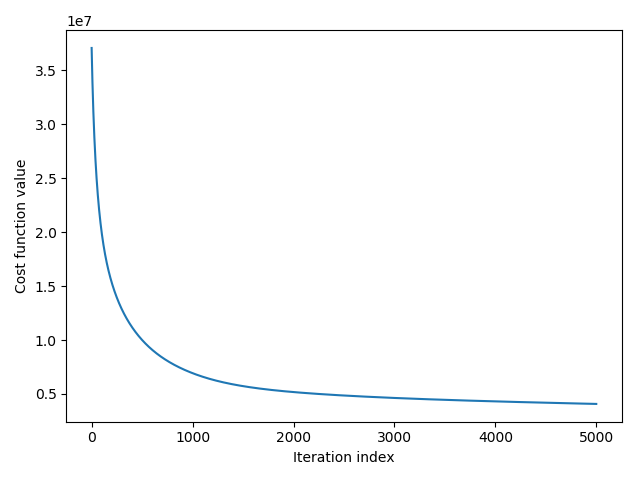
\includegraphics[width=\textwidth]{anmf_mdct_cost_func.png}
\end{figure}

Learning a lesson from the ANMF-RAW experiments, it's worth figuring out whether ANMF-MDCT is even practical at all. To do that, we need to be able to calculate the bitrate of ANMF-MDCT first. Assuming rank $r$, sampling rate $F_s$, frame size $S_f$ and chunk size $S_c$, our bitrate is:

\begin{align}
bitrate^{MDCT} &= r(\frac{S_f}{2} + S_c) \cdot \frac{F_s}{\frac12 S_fS_c} \cdot bitsPerValue \cdot channelCount
\end{align}

And as before, our initial goal is a target bitrate of 750 kbps. To achieve that, we either use a higher rank and higher chunk size, or vice versa.

First, I tried to fix the rank to a relatively high value, specifically $r = 60$. If we fill the known values into the equation and solve for $S_c$, we obtain a chunk size of $S_c \approx 371$. Similarly, if we go with a small chunk size, e.g. $S_c = 100$, we obtain a rank of $r \approx 23$.

However, as we can see in Table \ref{tab:anmf_mdct_rank}, the ODG values are less than usable (and it sounds terrible to my ears as well). This seems to be mostly due to the fact that the phase data contained in the MDCT coefficients is very sensitive to inaccuracies and throws the signal off.

Out of curiosity, I tried increasing the frame size as well, but this only led to the signal being unrecognizable and there doesn't seem to be a good reason to do it in the first place.

\begin{table}[htbp]\caption{ANMF-MDCT rank experiment results}
	\label{tab:anmf_mdct_rank}
	\centering
	\begin{tabular}{|c|c|c|}
		\hline
		ID & $r = 23, S_c = 100$ & $r = 60, S_c = 371$ \\ \hline
		$00$ & $-3.910$ & $-3.911$ \\
		$01$ & $-3.913$ & $-3.913$ \\
		$02$ & $-3.909$ & $-3.910$ \\
		$03$ & $-3.878$ & $-3.877$ \\		
		\hline
	\end{tabular}
\end{table}

Due to the fact that ANMF-MDCT did not produce usable results at a comparatively high bitrate, it will not be tested further.

\subsection{ANMF-STFT}
ANMF-STFT seemed to produce the best results during preliminary testing when I was implementing the codec, so given that and the large amount of parameters, this method will be tested thoroughly.

For baseline parameters that seemed to work well, we choose frame size $S_f = 1152$, chunk size $S_c = 500$, $\mu_W = 10^4$ and $\mu_H = 10^5$. On Figure \ref{fig:anmf_stft_cost_func} we notice NMF converges a lot sooner than in the previous methods, so we will set max iterations to only 1000.

\begin{figure}[ht]
	\caption[ANMF-STFT cost function]{The value of the cost function per iteration during NMF in ANMF-STFT at rank $= 40$. Logarithmic scale is used for better visibility.}
	\label{fig:anmf_stft_cost_func}
	\centering
	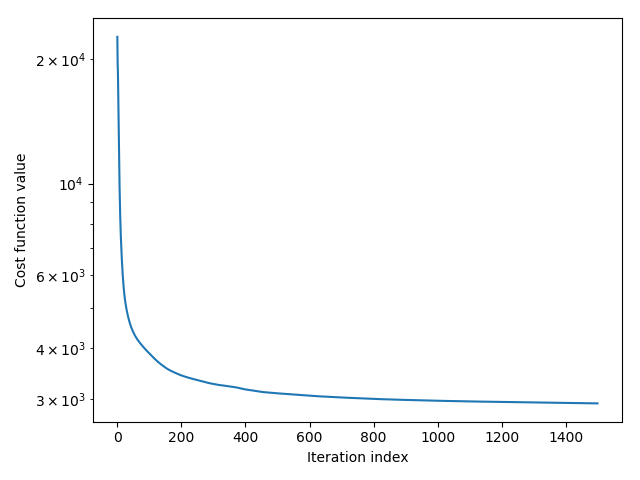
\includegraphics[width=\textwidth]{anmf_stft_cost_func.png}
\end{figure}

Calculating the bitrate here is going to be a bit different. Since we use Huffman coding, the bitrate will vary, since each value uses a different amount of bits, but we can still estimate it.

To estimate the "average" bitrate, we will take the Huffman table and interpret it as a random variable, specifically $X_P$ for the phase spectrogram and $X_H$ for the coefficient matrix of the magnitude spectrogram. As its output, we'll use the amount of bits necessary to encode a value. For the probability distribution of these values, we can use the data we obtained before as seen in Figures \ref{fig:stft_phase_quant_freq} and \ref{fig:stft_quant_freq}. We then find the expected values $E[X_P]$ and $E[X_H]$ for each of them.

The expected value $E[X]$ of a discrete random variable $X$ is simply put an average of the possible values weighted by their respective probabilities. Formally, it is defined as \cite{Ross1972IntroductionTP}:

\begin{align}
E[X] = \sum_{i}x_ip_i
\end{align}

By applying this model to the Huffman tables, we find that $E[X_P] \approx 3.072$ bits, and $E[X_H] \approx 2.952$ bits. We can then proceed with bitrate calculation.

To calculate the bitrate of ANMF-STFT, it will be easiest to calculate the bits necessary for the phase matrix and the coefficient matrix separately, and then add them together. The equations are:

For the phase matrix:

\begin{align}
bits^{PHASE}
&= E[X_P] \cdot \frac{S_f}{2} \cdot \frac{F_s}{\frac12 S_f} \\
&= E[X_P] \cdot F_s
\end{align}

For the magnitude matrix:

\begin{align}
bits^W &= r \cdot S_c \cdot 32 \\
bits^H &= r \cdot \frac{S_f}{2} \cdot E[X_H] \\
bits^{MAG} &= (bits^W + bits^H) \cdot \frac{F_s}{\frac12 S_fS_c} \\
&= \left( r \cdot S_c \cdot 32 + r \cdot \frac{S_f}{2} \cdot E[X_H] \right) \cdot \frac{F_s}{\frac12 S_fS_c} \\
&= r(32 \cdot S_c + \frac{S_f}{2} \cdot E[X_H]) \cdot \frac{F_s}{\frac12 S_fS_c}
\end{align}

And finally:

\begin{align}
bitrate^{STFT} &= (bits^{PHASE} + bits^{MAG}) \cdot channelCount \\
&= (E[X_P] \cdot F_s + r(32 \cdot S_c + \frac{S_f}{2} \cdot E[X_H]) \cdot \frac{F_s}{\frac12 S_fS_c}) \cdot channelCount \\
&= \left( \frac{E[X_H] \cdot r}{S_c} + \frac{64 \cdot r}{S_f} + E[X_P] \right) \cdot F_s \cdot channelCount
\end{align}

Substituting the variables for our reference values, we end up with a bitrate of $\sim 487$ kbps, which is lower than the previous methods, but at the same time, subjectively speaking, it actually sounds fairly promising. The next step is to stabilize this bitrate while experimenting with the variables and measuring the quality. Once we find out the most influencing factors and end up with satisfactory audio quality, we can try lowering the bitrate further to try and match existing codecs.

.. TODO experiment, tables, ODG, etc. ..

\subsection{Comparison}
.. TODO calculate bitrate for the wav files ..
.. TODO compare the "best" from the previous 3 vs MP3/Opus ..
